\chapter{Diseño e implementación} % Main chapter title

\label{Chapter3} % Change X to a consecutive number; for referencing this chapter elsewhere, use \ref{ChapterX}

\definecolor{mygreen}{rgb}{0,0.6,0}
\definecolor{mygray}{rgb}{0.5,0.5,0.5}
\definecolor{mymauve}{rgb}{0.58,0,0.82}

%%%%%%%%%%%%%%%%%%%%%%%%%%%%%%%%%%%%%%%%%%%%%%%%%%%%%%%%%%%%%%%%%%%%%%%%%%%%%
% parámetros para configurar el formato del código en los entornos lstlisting
%%%%%%%%%%%%%%%%%%%%%%%%%%%%%%%%%%%%%%%%%%%%%%%%%%%%%%%%%%%%%%%%%%%%%%%%%%%%%
\lstset{ %
  backgroundcolor=\color{white},   % choose the background color; you must add \usepackage{color} or \usepackage{xcolor}
  basicstyle=\footnotesize,        % the size of the fonts that are used for the code
  breakatwhitespace=false,         % sets if automatic breaks should only happen at whitespace
  breaklines=true,                 % sets automatic line breaking
  captionpos=b,                    % sets the caption-position to bottom
  commentstyle=\color{mygreen},    % comment style
  deletekeywords={...},            % if you want to delete keywords from the given language
  %escapeinside={\%*}{*)},          % if you want to add LaTeX within your code
  %extendedchars=true,              % lets you use non-ASCII characters; for 8-bits encodings only, does not work with UTF-8
  %frame=single,	                % adds a frame around the code
  keepspaces=true,                 % keeps spaces in text, useful for keeping indentation of code (possibly needs columns=flexible)
  keywordstyle=\color{blue},       % keyword style
  language=[ANSI]C,                % the language of the code
  %otherkeywords={*,...},           % if you want to add more keywords to the set
  numbers=left,                    % where to put the line-numbers; possible values are (none, left, right)
  numbersep=5pt,                   % how far the line-numbers are from the code
  numberstyle=\tiny\color{mygray}, % the style that is used for the line-numbers
  rulecolor=\color{black},         % if not set, the frame-color may be changed on line-breaks within not-black text (e.g. comments (green here))
  showspaces=false,                % show spaces everywhere adding particular underscores; it overrides 'showstringspaces'
  showstringspaces=false,          % underline spaces within strings only
  showtabs=false,                  % show tabs within strings adding particular underscores
  stepnumber=1,                    % the step between two line-numbers. If it's 1, each line will be numbered
  stringstyle=\color{mymauve},     % string literal style
  tabsize=2,	                   % sets default tabsize to 2 spaces
  title=\lstname,                  % show the filename of files included with \lstinputlisting; also try caption instead of title
  morecomment=[s]{/*}{*/}
}
%----------------------------------------------------------------------------------------

En este capítulo se detallan los componentes de software y hardware diseñados e implementados por el autor, su interrelación, y los criterios seguidos.

%----------------------------------------------------------------------------------------
%	SECTION 1
%----------------------------------------------------------------------------------------
\section{Arquitectura del sistema}

Para abordar el trabajo realizado, en esta sección se expone la arquitectura general del sistema embebido implementado, esquematizada en el diagrama de la figura \ref{fig:diagramaCompleto}, y luego, en las siguientes secciones, se detallan cada uno de los componentes de manera individual.

\begin{figure}[htbp]
	\centering
	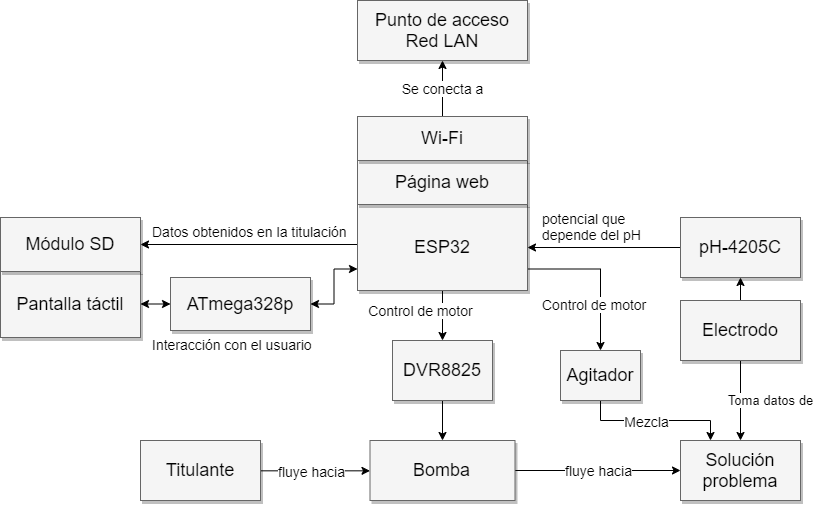
\includegraphics[width=1.0\textwidth]{./Figures/DiagramaBloquesCompleto.png}
	\caption{Diagrama en bloques del trabajo realizado.}
	\label{fig:diagramaCompleto}
\end{figure}

El componente principal del sistema es el ESP32, que tiene como función coordinar cada una de las partes intervinientes. A través de una comunicación del tipo UART con el ATmega328p, recibe las órdenes ingresadas a través de la pantalla táctil para realizar las configuraciones o funciones que solicite el usuario.

Dentro de las principales configuraciones, está la posibilidad de modificar el volumen de corte y de habilitar, o no, el agitador. El volumen de corte es la cantidad máxima de titulante que se utiliza durante la titulación. Cuando se alcanza ese valor, el proceso se detiene automáticamente. En cuanto a la habilitación del agitador, permite elegir si el mismo se activa, o no, al iniciar la titulación.

Las funciones principales que ofrece el sistema son las de limpieza, calibración y titulación. El modo limpieza se utiliza para purgar la bomba previo al proceso de titulación y para eliminar los retos de titulante que quedan en las mangueras al finalizar el proceso. 

La calibración permite ajustar el valor leído por el ADC, en el cual se encuentra conectado el módulo pH4502C. Para llevarla a cabo, se hace uso de tres líquidos patrones, denominados \textit{buffers}, de pH 4, 7 y 10, respectivamente. Se debe realizar la calibración de manera periódica, ya que las propiedades del electrodo varían con el tiempo.

Una vez realizadas las configuraciones correspondientes de limpieza y calibración, es posible iniciar la titulación. Cuando esto sucede, el ESP32 activa  la bomba para que comience a inyectar el titulante en la muestra problema, y registra los valores de pH asociados, que obtiene desde el electrodo. En la pantalla se visualiza una curva del pH a lo largo del tiempo, y se ofrece la posibilidad de finalizar el proceso mediante un botón, en el momento que el usuario lo desee. En caso contrario, el proceso finaliza al alcanzar el volumen de corte.

Luego, el ESP32 calcula la derivada primera para cada valor de volumen y pH asociados, y, en base a ello, encuentra la cantidad de volumen inyectado en el punto final. Tanto este resultado, como todos los valores registrados, se almacenan en la memoria micro SD, a través de una comunicación SPI con el módulo correspondiente, y en la página web, que se encuentra embebida en la memoria del ESP32. A través de una conexión de área local, se puede acceder a esta página desde otro dispositivo y visualizar los resultados.

Para realizar las actividades mencionadas previamente, el ESP32 ejecuta tres tareas: la tarea encargada de la comunicación UART con el ATmega328p, que se aloja en el núcleo 0, y las tareas de medición del electrodo y de control de la bomba, que se alojan en el núcleo 1. Además, existe un controlador de eventos, que se ejecuta sobre el núcleo 0 cuando alguien accede a la página web.


%----------------------------------------------------------------------------------------
\section{Medición del electrodo}

La medición del electrodo es un módulo de software que implementa una tarea de FreeRTOS. El objetivo de esta tarea es obtener el valor del conversor ADC, que proviene del módulo pH-4502C, y es ejecutada durante los procesos de calibración y de titulación. En el código \ref{cod:tareaElectrodo} se muestra el pseudocódigo de la tarea de medición del electrodo. Al inicio de esta tarea se realiza la configuración del ADC utilizado, el cual se habilita con una resolución de 12 bits en el pin correspondiente al canal 6 del ADC número 1.

La lectura del valor del ADC se acumula en la variable sumaAdc durante las N iteraciones del bucle \textit{for}. Cada una de estas iteraciones se realiza en un intervalo de 10 mS, y, al finalizar el bucle \textit{for}, el valor total se divide por la cantidad de muestras realizadas, lo que permite promediar el valor leído y así reducir el ruido presente en la conversión, tal y como sugiere la página oficial del ESP32 \citep{WEBSITE:2}. Cabe destacar que el acceso a la variable valorAdc está protegido por una sección crítica, ya que el resto de las tareas también pueden acceder a la variable cuando precisan calcular el valor de pH.

\begin{lstlisting}[label=cod:tareaElectrodo,caption=Pseudocódigo de la tarea de medición de pH.]
void tareaElectrodo (void *arg)
{
    //Configuracion de resolucion y pin del ADC
    configuracionADC(12 bits, pin);
    uint32_t sumaAdc = 0;

    while(true)
    {
    for (int i=0; i< N_MUESTRAS; i++)
    {
        sumaAdc = sumaAdc + lecturaADC(pin);  
        vTaskDelay(10 mS);
    } 
    inicioSeccionCritica(); 
    valorAdc = sumaAdc / N_MUESTRAS;
    finSeccionCritica();
    sumaAdc = 0;
    }
}
\end{lstlisting}

%----------------------------------------------------------------------------------------
\section{Proceso de calibración}

En todo equipo de medición, es importante asegurar que los valores sean confiables a lo largo del tiempo. Debido a que las propiedades de los electrodos varían a lo largo de su vida útil, es fundamental que un titulador automático disponga de un proceso de calibración que permita realizar los ajustes necesarios de manera periódica.

La calibración de electrodos de pH se realiza mediante la utilización de \textit{buffers}, que son patrones de medición en estado líquido, de pH 4, 7 y 10. Esto permite asociar el potencial que entrega el electrodo a su valor de pH correspondiente y crear la ecuación de la recta que mejor se ajuste a estos tres puntos, ya que, como se menciona en la ecuación \ref{eq:phElectrodo} del capítulo \ref{Chapter2}, el valor de pH de la muestra es inversamente proporcional a la diferencia de potencial que entrega el electrodo, para este caso en particular, el modelo HANNA HI-1230B.

En este trabajo se incluye un proceso de calibración, que el usuario puede acceder desde el menú de la pantalla táctil, para realizar la calibración con cada uno de los tres patrones mencionados. Para ello, el electrodo debe estar en contacto con el \textit{buffer} durante unos segundos hasta que el valor de la medición se estabilice, y, en ese momento, el usuario puede guardar el valor leído por el ADC, el cual queda asociado al valor de pH del patrón utilizado. Una vez realizado el proceso para los tres \textit{buffers}, se obtienen tres puntos con los cuales se puede construir la recta de regresión, que es la recta que mejor se ajusta a estos tres puntos. De este cálculo, surge la pendiente m y la ordenada al origen b, que son valores que se almacenan en la memoria flash no volátil del ESP32, y se utilizan en la ecuación \ref{eq:conversionPh}. Está ecuación se ejecuta cada vez que el ESP32 necesita convertir la variable valorADC a un valor de pH.

\begin{equation}
	\label{eq:conversionPh}
pH = m * valorAdc + b
\end{equation}


%----------------------------------------------------------------------------------------
\section{Control de la bomba}

El control de la bomba se realiza a través del \textit{driver} DVR8825, que maneja al motor paso a paso, y, mediante hardware, fue configurado con el \textit{microsteping} en 1/32. Esto significa que el motor debe realizar 6400 micropasos para producir un giro completo. Los pines de dirección y de paso están conectados a dos pines del ESP32. El pin de dirección fue configurado mediante software para producir el sentido de giro que permite desplazar el titulante desde su recipiente hasta el recipiente de la muestra. En cuanto al pin de paso, este es controlado por PWM, que genera una onda cuadrada de 10 KHz. Esto se traduce a una velocidad de 93,74 rpm en el eje del motor.

Las configuraciones de software mencionadas anteriormente se realizan al inicio la tarea de control de la bomba, en el bloque correspondiente a configuración de PWM del diagrama que muestra la figura \ref{fig:flujoBomba}.

Una vez realizadas las configuraciones, la tarea de control de la bomba tiene la posibilidad de ejecutar dos funciones según lo que decida el usuario a través de la pantalla táctil. Una de las opciones es el proceso de limpieza, en el cual simplemente se activa la bomba, es decir, se habilita el PWM que produce la onda cuadrada que llega al pin de paso del DVR8825 y genera el giro del motor. Este proceso se ejecuta hasta que el usuario decida detenerlo.

La otra función corresponde al proceso de titulación. El requerimiento TPA-ERS-01-REQ012 establece que es necesario inyectar 0,1 mL y luego realizar una espera de 5 segundos antes de realizar la medición de pH. Esta cantidad de volumen se logra cuando el motor produce 11500 micropasos, lo que equivale a que el PWM esté activado durante 1150 ms, valor definido mediante la etiqueta T-CORTO. Además, el requerimiento contempla que, para cuando la variación de pH entre dos mediciones  sea menor a 0,2, se puede inyectar 1 mL en lugar de 0,1 mL, por lo cual se define la etiqueta T-LARGO en 11500 ms. Esto es útil para agilizar el proceso, especialmente al inicio de la titulación, donde el pH varía de manera lenta a medida que se agrega volumen, como se mostró anteriormente en la figura \ref{fig:sigmoidea}. Las pruebas que permitieron llegar a estos valores son mencionadas en el capítulo \ref{Chapter4}.

\begin{figure}[htbp]
	\centering
	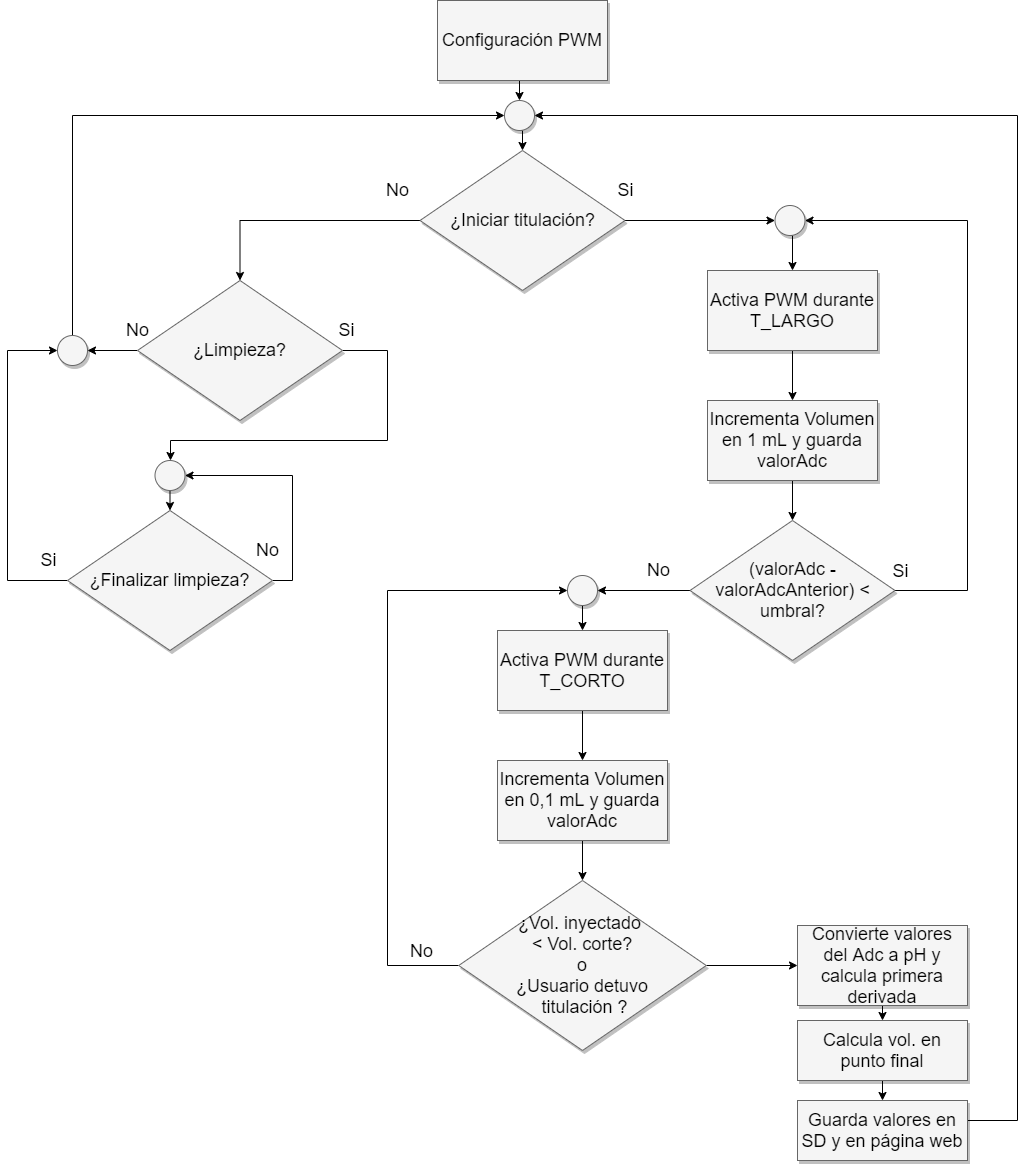
\includegraphics[width=1.0\textwidth]{./Figures/motorBomba.png}
	\caption{Diagrama de flujo de la tarea de control de la bomba.}
	\label{fig:flujoBomba}
\end{figure}

Ya definidas las configuraciones y los tiempos para cada cantidad del volumen, el proceso de titulación inicia con la activación del PWM que produce el giro de la bomba hasta alcanzar la cantidad de 1 mL de titulante inyectado. Llegado a este punto, se produce una espera de 5 segundos y luego, el valor leído por la tarea del electrodo se almacena en un arreglo, al igual que la cantidad de volumen acumulado. El proceso se repite hasta que la diferencia entre las dos ultimas mediciones del electrodo supere un umbral, equivalente a aproximadamente 0,2 de pH. A partir de este momento, se modifica la cantidad de volumen inyectado a 0,1 mL, pero el resto del procedimiento es el mismo. Una vez alcanzado el volumen de corte, o si el usuario presiona el boton de finalizar, la bomba se detiene y se llama a una función que calcula el valor de pH para cada valor almacenado en el arreglo de mediciones del electrodo. Luego, se calcula el valor de la primera derivada del pH respecto al volumen para cada uno de los valores del arreglo y se determina el volumen en el punto final en base al valor máximo de la primera derivada. Todos los valores son almacenados en la memoria micro SD y en la página web, para que el usuario pueda tener acceso, y el valor de volumen en el punto final es mostrado en la pantalla.


%----------------------------------------------------------------------------------------
\section{Interfaz de usuario}

La interfaz de usuario permite el acceso a todas las configuraciones y funciones que presenta el titulador. Está implementada a través de una pantalla táctil que permite navegar por un menú de diferentes pantallas, que fueron implementadas mediante la máquina de estados de la figura \ref{fig:MEFmenu}.

La máquina de estados se ejecuta en el ATMega328p y cada estado tiene una pantalla gráfica asociada con botones táctiles que permiten navegar entre las diferentes opciones. Por ejemplo, desde el menú inicial se puede acceder al menú de titulación a través del botón TITULAR.

\begin{figure}[htbp]
	\centering
	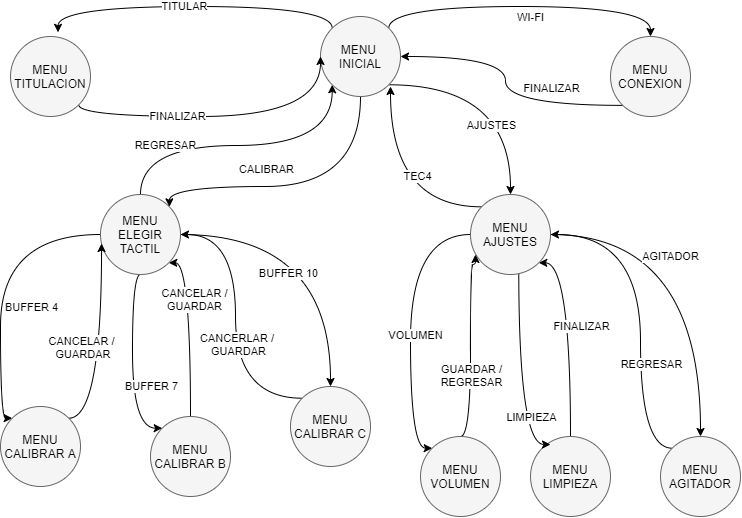
\includegraphics[width=1.0\textwidth]{./Figures/MEFmenu.png}
	\caption{Máquina de estados del menú de usuario.}
	\label{fig:MEFmenu}
\end{figure}

A continuación se listan las características de cada uno de los estados:

\begin{itemize}
\item Menú inicial: es el estado en el cual se ingresa cuando se inicia el programa. Desde aquí se puede acceder a la calibración, a la titulación, al menú de ajustes y al menú de conexión.
\item Menú elegir \textit{buffer}: se utiliza para elegir el \textit{buffer}  con el cual se desea calibrar. Para completar el proceso de calibración de manera correcta, se debe ingresar en cada uno de los tres \textit{buffers}. Al presionar REGRESAR se envía por UART que el proceso de calibración finalizó para que el ESP32 actualice la función correspondiente al cálculo del valor de pH.
\item Menú calibrar A: es el estado en el cual se calibra usando el \textit{buffer} de pH 4. En este estado el ATmega328p se comunica con el ESP32 para solicitarle el valor actual de pH. Este valor sirve como referencia para que el usuario presione GUARDAR una vez que la lectura sea estable. Al presionar GUARDAR, se envía la confirmación al ESP32 para que actualice el valor correspondiente al \textit{buffer} de pH 4, y se regresa al menú de elegir \textit{buffer}. En caso de presionar regresar, vuelve al menú pero sin enviar la confirmación al ESP32.
\item Menú calibrar B: es el estado en el cual se calibra usando el \textit{buffer} de pH 7, y sigue el mismo procedimiento que el menú calibrar A.
\item Menú calibrar C: es el estado en el cual se calibra usando el \textit{buffer} de pH 10, y sigue el mismo procedimiento que el menú calibrar A.
\item Menú titulación: es el estado en el cual se realiza el proceso de titulación, por ende, se envía un comando al ESP32 para que se ejecute la función de titulación dentro de la tarea de la bomba.
\item Menú ajustes: es el estado que permite acceder a varias configuraciones.
\item Menú volumen: es el estado que permite seleccionar el volumen de corte. Cuando se ingresa a este, se envía un comando al ESP32 para consultar el volumen de corte actual y mostrarlo en pantalla. Mediante un botón + y otro botón - se puede variar de a 1 mL este valor. Luego al presionar GUARDAR se envía el nuevo valor al ESP32, mientras que si se presionar REGRESAR vuelve al menú anterior sin hacer cambios.
\item Menú limpieza: es el estado que permite purgar o limpiar las mangueras de la bomba.  Aquí se envía un comando al ESP32 para que ejecute la función de limpieza dentro de la tarea de la bomba.
\item Menú agitador: es el estado que permite habilitar o deshabilitar el uso del agitador. Tiene los botones ON y OFF que envian al ESP32 el comando correspondiente para activar o desactivar el agitador respectivamente.
\item Menú conexión: es el estado que permitirá, en futuras versiones, acceder a configuraciones de la conexión Wi-Fi. Actualmente muestra la pantalla correspondiente pero no ejecuta ninguna acción.
\end{itemize}

Como se mencionó anteriormente, la máquina de estados funciona dentro del ATmega328p y en algunos estados se produce una comunicación del tipo UART con el ESP32 para el intercambio de la información necesaria. Esta comunicación se realiza mediante comandos que representan determinadas acciones, algunos de los cuales van acompañados de algún valor o requieren determinada respuesta. A continuación, se describe cada uno de los comandos implementados:

\begin{itemize}
	\item Comando ''A'': El ATmega328p le indica al ESP32 que inicie el proceso de calibración.
	\item Comando ''B'': El ATmega328p le indica al ESP32 que finalice el proceso de calibración. El ESP32 calcula el coeficiente y la ordenada al origen la ecuación que convierte el valor leído por el ADC a pH.
	\item Comando ''C'': El ATmega328p le indica al ESP32 que convierta el valorAdc a pH y lo devuelva como respuesta.
	\item Comando ''D'': El ATmega328p le indica al ESP32 que el usuario guarde el valor actual de valorAdc como valor de calibración del \textit{buffer} de pH 4.
	\item Comando ''E'': El ATmega328p le indica al ESP32 que el usuario guarde el valor actual de valorAdc como valor de calibración del \textit{buffer} de pH 7.
	\item Comando ''F'': El ATmega328p le indica al ESP32 que el usuario guarde el valor actual de valorAdc como valor de calibración del \textit{buffer} de pH 10.
	\item Comando ''G'': El ATmega328p le indica al ESP32 que inicie el proceso de titulación.
	\item Comando ''I'': El ATmega328p le indica al ESP32 que finalice el proceso de titulación, porque el usuario lo seleccionó.  
	\item Comando ''J'': El ESP32 le indica al ATmega328p le indica al ESP32 el proceso de titulación finalizó, porque se alcanzó el volumen de corte.
	\item Comando ''K'': El ATmega328p le indica al ESP32 que inicie el proceso de limpieza.
	\item Comando ''L'': El ATmega328p le indica al ESP32 que finalice el proceso de limpieza.
	\item Comando ''M'': El ATmega328p le indica al ESP32 devuelva como respuesta el valor actual de volumen de corte.
	\item Comando ''N'': El ATmega328p le envía al ESP32 el valor de volumen de corte ingresado por el usuario.
	\item Comando ''P'': El ATmega328p le indica al ESP32 que habilite el agitador.
	\item Comando ''Q'': El ATmega328p le indica al ESP32 que deshabilite el agitador.
\end{itemize}



%----------------------------------------------------------------------------------------
\section{Almacenamiento de datos}

El almacenamiento de datos es una característica importante en este tipo de dispositivos ya que permite registrar los resultados de cada titulación para su posterior análisis en una computadora. Como método de almacenamiento, se decidió utilizar una memoria del tipo micro SD, para sacar provecho del módulo que trae integrado la placa MCUFRIEND.

La API ESP-IDF incorpora funciones de alto nivel para la configuración, lectura y escritura de memorias SD a través del bus SPI. Para este trabajo se creó un módulo de software, formado por un archivo denominado sd.c asociado al archivo sd.h, que ofrece funciones para inicializar la SD y escribir en ella.

La función inicializarSD se llama al inicio desde la función principal, previo a la creación de tareas, y hace la configuración inicial para habilitar el uso de la memoria micro SD. Dentro de ella, se hace el llamado a  la función spi\_bus\_initialize que inicia el bus SPI con las configuraciones de pines y velocidad, entre otras, necesarias para la comunicación. Luego se realiza el llamado a esp\_vfs\_fat\_sdspi\_mount que especifica que sobre el bus SPI se monta una memoria del tipo SD que funciona con el sistema de archivos FAT.

La función para escribir en el archivo es accedida desde la tarea de la bomba para almacenar los datos correspondientes al volumen inyectado y pH, y, además, el resultado del volumen en el punto final. El detalle de esta función se muestra en el pseudocódigo \ref{cod:escribeSD}, donde se observa que se abre un archivo, y en caso de que no se produzca un error, se procede a la escritura, y, finalmente, se cierra el archivo.

\begin{lstlisting}[label=cod:escribeSD,caption=Pseudocódigo de la función que escribe en la memoria SD.]
    FILE* f = fopen("TITULAR.txt", "a"); //Abre el archivo
    if (f == NULL) {
        return ERROR;
    }
    fprintf(f, "%s",dato);
    fclose(f);
    return OK;
\end{lstlisting}



%----------------------------------------------------------------------------------------
\section{Servidor web}

Para el desarrollo del prototipo, se elaboró una página web que se almacena en la memoria flash del ESP32, y que se puede acceder a través de una conexión de área local gracias a la conexión Wi-Fi de la que dispone el módulo. En el código \ref{cod:servidorWeb} se muestra el pseudocódigo donde se encuentran las principales funciones que se utilizan para la conexión Wi-Fi y para la creación del servidor web.

La función iniciarWiFi se encarga de habilitar la conexión Wi-Fi en modo estación, con el nombre de la red y la contraseña del punto de acceso al cual se desea conectar. Por último, registra eventos que se ejecutan cuando hay un cambio de ip o se produce un corte en la conexión, y tienen como objetivo restablecer la conexión.

La función iniciarServidorWeb inicia un servidor HTTP con configuraciones por defecto que ofrece la API, y registra un evento asociado a la página web. Este evento se ejecuta cuando un cliente, conectado a la red local, intenta establecer la conexión mediante la ip asociada al ESP32. El controlador del evento ejecuta la función que actualiza la página web con los datos obtenidos en el último proceso de titulación.


\begin{lstlisting}[label=cod:servidorWeb,caption=Pseudocódigo del servidor web.]
main (){
	//...
	iniciarWiFi();
	iniciarServidorWeb();
	//...
}

//...

void iniciarWiFi()
{
	esp_wifi_init(); //Inicializa el stack de Wi-Fi con configuraciones por defecto
	esp_wifi_set_mode(ESTACION); //Configura el modo estacion
	esp_wifi_set_config(wifi_config); //Configura nombre de red del AP y contrasena
	esp_wifi_start(); //Realiza la conexion Wi-Fi
	registraHandlerDeEventos();
}

iniciarServidorWeb()
{
	if(httpd_start(configuraciones) = OK) //Crea un servidor HTTP
	{
		httpd_register_uri_handler(paginaHandler); //registra una pagina
	}
	
}

paginaHandler() //evento que se ejecuta cuando alguien accede a la pagina
{
	//Codigo HTML de la pagina que contiene el volumen en el punto final
	//y una tabla del volumen inyectado y pH
}

\end{lstlisting}


%----------------------------------------------------------------------------------------
\section{Esquemáticos y PCB}

El diseño de los esquemáticos y del circuito impreso fueron realizados mediante la herramienta Kicad. En la figura \ref{fig:esquematicoESP} se observan la fuente de alimentación y las conexiones asociadas al ESP32. La fuente de alimentación consta de un regulador de tensión de 5 V, y su entrada proviene de una fuente externa de 12 V de corriente continua.

El ESP32 se conecta al módulo pH4502C mediante divisores resistivos para adaptar tensiones. Utiliza dos pines GPIO para la conexión al módulo DVR8825, un pin GPIO para la conexión al driver del agitador, cuatro pines asociados a la conexión para la comunicación SPI con el módulo lector de tarjetas micro SD, y dos pines para la comunicación UART con el ATmega328p. Además, los pines sin usado están conectados a tiras de pines para aplicaciones futuras.

\begin{figure}[htbp]
	\centering
	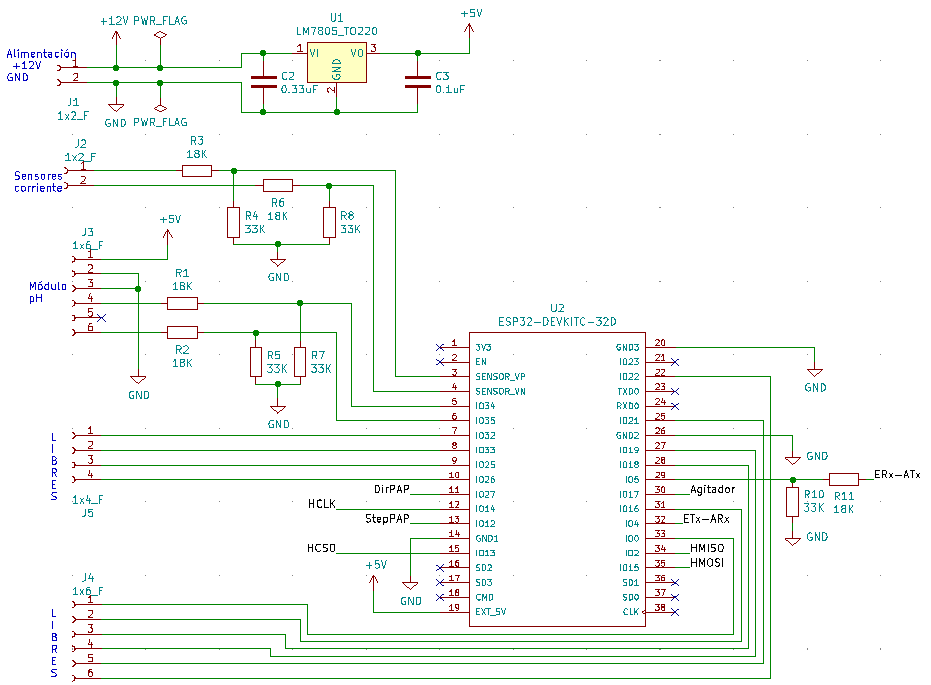
\includegraphics[width=1.0\textwidth]{./Figures/esquematicoESP.png}
	\caption{Diseño esquemático de las conexiones del ESP32.}
	\label{fig:esquematicoESP}
\end{figure}

La figura \ref{fig:esquematicoAtmega} muestra las conexiones del ATmega328p con los pines de control y datos de la pantalla táctil, asi como también los componentes mínimos necesarios para el funcionamiento del microcontrolador.

\begin{figure}[htbp]
	\centering
	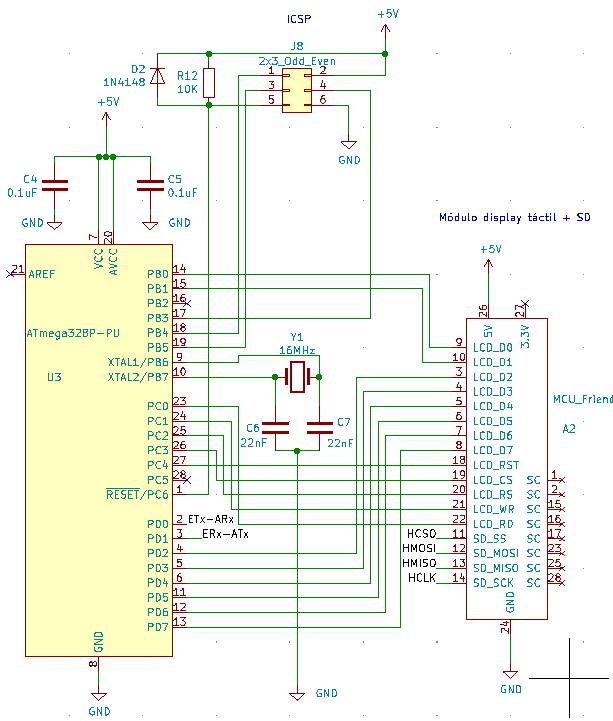
\includegraphics[width=0.6\textwidth]{./Figures/esquematicoAtmega.png}
	\caption{Diseño esquemático de las conexiones del ATmega328p.}
	\label{fig:esquematicoAtmega}
\end{figure}

El \textit{driver} DVR8825 tiene conectado un \textit{dip switch} que permite establecer por hardware el valor de configuración de \textit{microsteping}. Además, tiene el conector para los cables de las bobinas del motor. El \textit{driver} del agitador está formado por un transistor BJT en configuración común. Estos circuitos están representados en la figura \ref{fig:esquematicoMotores}.

\begin{figure}[htbp]
	\centering
	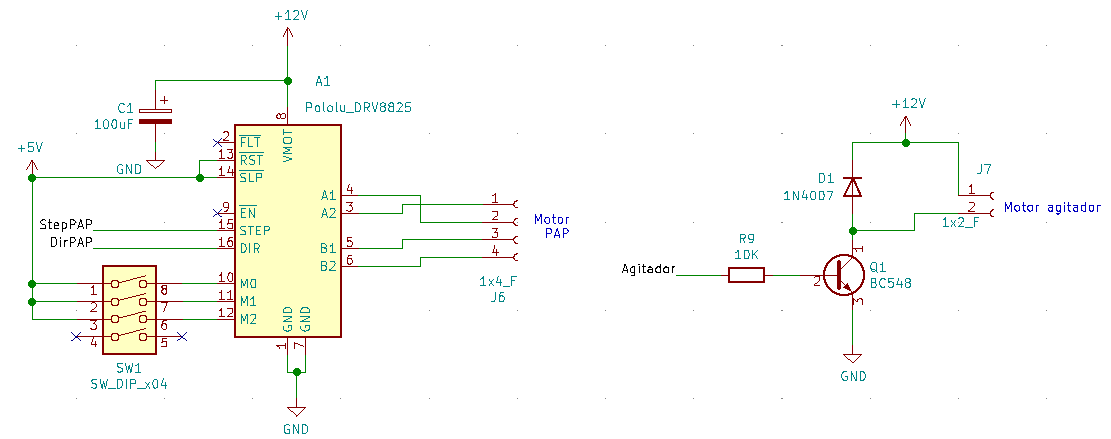
\includegraphics[width=1.0\textwidth]{./Figures/esquematicoMotores.png}
	\caption{Diseño esquemático de los drivers de la bomba y del agitador.}
	\label{fig:esquematicoMotores}
\end{figure}

El circuito impreso es una placa 75 x 150 mm de dimensiones, diseñada en simple faz, y tiene como función la conexión de todos los módulos utilizados. En la figura \ref{fig:pcb} se muestra el diseño del PCB, mientras que en la figura \ref{fig:pcb3D} se observa el modelo 3D.

\begin{figure}[htbp]
	\centering
	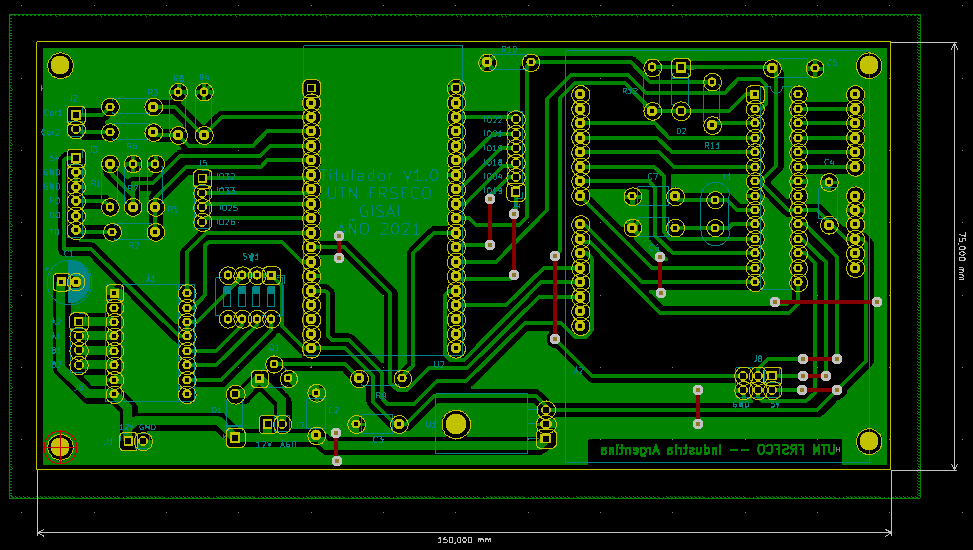
\includegraphics[width=1.0\textwidth]{./Figures/pcb.png}
	\caption{Diseño del PCB.}
	\label{fig:pcb}
\end{figure}

\begin{figure}[htbp]
	\centering
	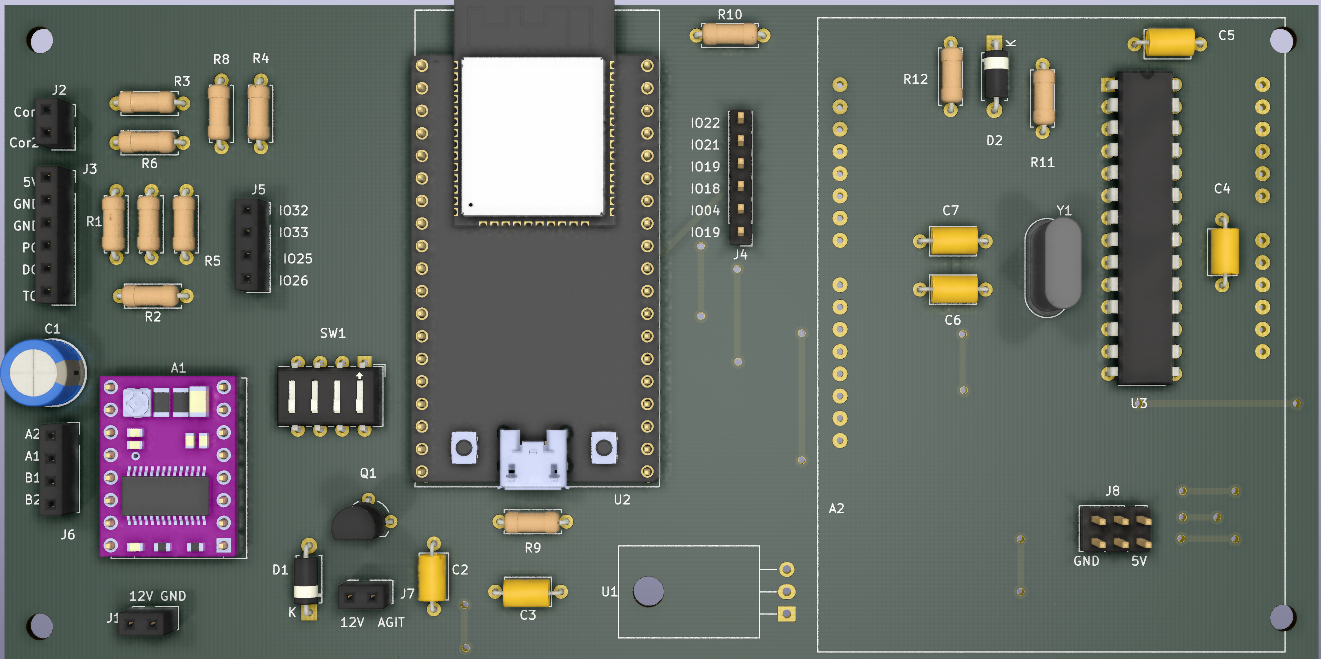
\includegraphics[width=1.0\textwidth]{./Figures/pcb3D.png}
	\caption{Modelo 3D del PCB.}
	\label{fig:pcb3D}
\end{figure}
